\section{Target-adapted geometry: theory, protocol, and complete results}
\label{app:target-geometry}

\subsection{Residual-target transport between fitted baselines}
\label{app:target-transport}

The following projection identity distinguishes residuals of a donor
baseline from residuals of the final baseline. Condition on the fitted
state, including a measurable representation
$\Gamma:\R^d\to\R^p$ and two predictors
$f_0,f_d:\R^d\to\R^H$. Let $(X,Y)$ be a fresh evaluation pair,
write $Z=\Gamma(X)$, and assume that $Y$, $f_0(X)$, and $f_d(X)$
have finite second moments. All expectations below refer to this
conditional evaluation distribution. For a fixed symmetric
positive-definite matrix $W\in\R^{H\times H}$, define
\[
 \langle a,b\rangle_W=a^\top Wb,\qquad
 \|a\|_W^2=a^\top Wa,\qquad
 R_W(f)=\E\|Y-f(X)\|_W^2.
\]
Here $a,b\in\R^H$. The equal-coordinate mean squared loss uses
$W=I_H/H$, where $I_H$ is the $H$-dimensional identity matrix.

\begin{proposition}[Correction gain and donor mismatch]
\label{prop:target-transport}
Define the conditional residual and conditional donor discrepancy by
\[
 m_0(Z)=\E[Y-f_0(X)\mid Z],\qquad
 b_d(Z)=\E[f_0(X)-f_d(X)\mid Z].
\]
For every measurable correction $q:\R^p\to\R^H$ satisfying
$\E\|q(Z)\|_2^2<\infty$,
\begin{equation}
 R_W(f_0)-R_W(f_0+q\circ\Gamma)
 =\E\|m_0(Z)\|_W^2-\E\|q(Z)-m_0(Z)\|_W^2.
 \label{eq:target-general-gain}
\end{equation}
The donor's optimal population correction is
$q_d(Z)=\E[Y-f_d(X)\mid Z]=m_0(Z)+b_d(Z)$. Hence
\begin{align}
 R_W(f_0)-R_W(f_0+q_d\circ\Gamma)
 &=\E\|m_0(Z)\|_W^2-\E\|b_d(Z)\|_W^2,
 \label{eq:target-transport-proof}\\
 R_W(f_0)-R_W(f_0+\widehat q\circ\Gamma)
 &=\E\|m_0(Z)\|_W^2-\E\|b_d(Z)+a(Z)\|_W^2,
 \label{eq:target-fitted-transport}
\end{align}
where $\widehat q$ is any square-integrable fitted correction and
$a(Z)=\widehat q(Z)-q_d(Z)$. Moreover,
\[
 \E\|b_d(Z)\|_W^2\leq\E\|f_0(X)-f_d(X)\|_W^2.
\]
\end{proposition}

\begin{proof}
Set $\epsilon=Y-f_0(X)-m_0(Z)$. By the definition of conditional
expectation, $\E[\epsilon\mid Z]=0$. Because $m_0(Z)-q(Z)$ is
measurable with respect to $Z$ and $W$ is fixed,
\[
 \E\langle\epsilon,m_0(Z)-q(Z)\rangle_W
 =\E\langle\E[\epsilon\mid Z],m_0(Z)-q(Z)\rangle_W=0.
\]
Expanding the squared norm of
$Y-f_0(X)-q(Z)=\epsilon+m_0(Z)-q(Z)$ therefore gives
\[
 R_W(f_0+q\circ\Gamma)
 =\E\|\epsilon\|_W^2+\E\|m_0(Z)-q(Z)\|_W^2.
\]
Set $q=0$ in this equality and subtract the general expression to
obtain Equation~\eqref{eq:target-general-gain}. Linearity of conditional
expectation gives
$q_d(Z)=m_0(Z)+b_d(Z)$. Substituting this correction proves
Equation~\eqref{eq:target-transport-proof}; substituting
$\widehat q(Z)=q_d(Z)+a(Z)$ proves
Equation~\eqref{eq:target-fitted-transport}.
Finally, the function $v\mapsto v^\top Wv$ is convex. Conditional
Jensen's inequality yields
\[
 \|\E[f_0(X)-f_d(X)\mid Z]\|_W^2
 \leq\E[\|f_0(X)-f_d(X)\|_W^2\mid Z].
\]
Taking expectations proves the bound on donor discrepancy.
\end{proof}

The final term in Equation~\eqref{eq:target-fitted-transport} contains
$2\E\langle b_d,a\rangle_W$. It cannot be replaced by separate
nonnegative mismatch and estimation penalties without another
orthogonality argument: approximation error may reinforce or partially
cancel the donor discrepancy. Even an exact donor correction can harm
the final base when its conditional mismatch exceeds the final base's
predictable residual signal.

For fixed square-integrable donors $f_1,\ldots,f_K$ and deterministic weights
$\pi_k\geq0$ summing to one, let $\bar f=\sum_k\pi_k f_k$.
Expanding around $\bar f$ gives
\[
 \sum_k\pi_k\E\|Y-f_k(X)-q(Z)\|_W^2
 =\E\|Y-\bar f(X)-q(Z)\|_W^2
  +\sum_k\pi_k\E\|f_k(X)-\bar f(X)\|_W^2.
\]
The cross term vanishes because the weighted donor deviations sum to
zero. Hence the common-law population optimizer is
$\E[Y-\bar f(X)\mid Z]$, and the proposition applies with
$f_d=\bar f$. This does not identify a finite OOF fit with that
optimizer. Chronological folds can have different laws and sample
sizes; a donor index depending on the observation must retain that
joint law rather than being replaced by constant mixture weights.

For a fixed realized correction $\delta(X)$ satisfying
$\E\|\delta(X)\|_2^2<\infty$, direct expansion also gives
\begin{equation}
 R_W(f_0)-R_W(f_0+\delta)
 =2\E\langle Y-f_0(X),\delta(X)\rangle_W
  -\E\|\delta(X)\|_W^2.
 \label{eq:target-alignment-audit}
\end{equation}
A separately implemented verification program checks its empirical
counterpart from saved test predictions. It does not estimate the oracle $m_0$ or $b_d$.
Donor/final disagreement is recorded separately on correction-training
rows. The final baseline has seen those rows, so this diagnostic is not
an unbiased estimate of future disagreement or predictive risk.

\subsection{Evaluation protocol and source roster}
\label{app:target-protocol}

The executable protocol is \path{extensions/target_geometry/PROTOCOL.md};
its configuration, numerical dependencies, implementation, and prepared
input roster were hashed before the full evaluation. Development checks use separate
seeds and do not enter confirmation. The synthetic seeds are
11200--11211. For law index $l$ and split index $s=0,1,2$, the generator in Appendix~\ref{c:app:methods} receives the first state value from
\texttt{SeedSequence([seed,l,s,9027])}. Each task has 128/64/128
training/validation/test episodes of length 72, history 12, offsets
$1,4,12$ and stride four, yielding 13 origins per episode.
Observation generation follows the same law-specific conventions as
the controlled study.

For synthetic OOF targets, episode index modulo four assigns folds.
Each donor excludes every row of the queried episodes. Within its
remaining episodes, the first 80\% of ordered episode IDs fit its
inner candidate models and the rest select its penalty. The selected
donor is then fitted on all donor episodes. No queried episode or
outer-validation target selects that donor's penalty.

For natural series, the first $\lceil0.4n\rceil$ capped training origins
initialize the donor history; the remainder form three contiguous query
blocks. If $t_b$ is the first query origin, only donor rows with
$t+H\leq t_b$ are allowed. An 80/20 inner chronological split applies
the same target-availability condition before inner validation.
Fewer than eight inner-fitting rows invokes the predefined donor
penalty one. Fewer than eight outer donor rows makes that query block
ineligible for \emph{both} residual-target procedures. The fitting
sample is otherwise fixed by indices, not by residual values or model
success. Fewer than eight eligible correction rows retains the available
baselines and sends the correction arms to their declared ridge fallback.
An eligible donor fit failure sends its dependent methods to that
fallback. An unavailable primary base or required evaluation split is
retained as a task failure.

\begin{table}[!htbp]
\centering\small\setlength{\tabcolsep}{4pt}
\caption{Archive collections and fixed target-geometry roster.
$L$ is history length, $H$ the number of consecutive target steps, and
$p$ the seasonal period. Selection uses only training-prefix eligibility
and identifier hashes. These are 12 series from four selected collections,
not 12 independent application domains.}
\label{tab:target-roster}
\begin{tabular}{llrrrl}
\toprule
Collection & Frequency & $L$ & $H$ & $p$ & Selected series \\
\midrule
Australian electricity & Half-hourly & 48 & 12 & 48 & T3, T5, T1 \\
Bitcoin indicators & Daily & 28 & 7 & 7 & \begin{tabular}[t]{@{}l@{}}sent\_addresses, confirmation\_time,\\block\_size\end{tabular} \\
Melbourne pedestrian & Hourly & 48 & 6 & 24 & T10, T14, T20 \\
KDD2018 air quality & Hourly & 48 & 6 & 24 & T239, T99, T233 \\
\bottomrule
\end{tabular}
\end{table}

The source records are respectively
\href{https://doi.org/10.5281/zenodo.4659727}{10.5281/zenodo.4659727},
\href{https://doi.org/10.5281/zenodo.5121965}{10.5281/zenodo.5121965},
\href{https://doi.org/10.5281/zenodo.4656626}{10.5281/zenodo.4656626}, and
\href{https://doi.org/10.5281/zenodo.4656719}{10.5281/zenodo.4656719}.
All selected archive versions declare CC BY 4.0; archive/member hashes, attribution,
source exclusions and metadata are retained in
\path{extensions/target_geometry/sources/manifest.json}.
Bitcoin selections are activity indicators, not price forecasts.
These collections broaden source coverage but are not sampled randomly
from application domains. The study uses fixed archive versions and
does not reconstruct historical data-release vintages.

Training-prefix eligibility requires 96 finite windows and a positive
seasonal-difference mean-square scale, with first-difference fallback.
The selection salt is
\texttt{kahm-target-geometry-new-collections-v1}. Each series uses
chronological 60/20/20 splits. Training is capped at 512 windows and
validation/test at 64 origins per segment by even index spacing.
All targets lie inside their segment; later test histories can contain
already observed test values. Missing windows are excluded without
interpolation, defining an available-window estimand. The loss scale
uses the initial training prefix only. The naive control uses the
declared seasonal lag with an available-value fallback; synthetic
naive prediction is persistence.

The 18 primary contrasts use 12 paired repetition-level means each.
For positive differences favoring the second method, they compare
ridge with learned-OOF KAHM; identity-OOF KAHM with learned-OOF KAHM;
identity-in-sample KAHM with identity-OOF KAHM; and learned-OOF affine,
locality, and RBF-local with learned-OOF KAHM. For paired differences $d_1,\ldots,d_{12}$, let $\bar d$ be their
mean and $s_d$ their sample standard deviation. The interval is
$\bar d\pm t_{11,1-0.05/(2\cdot18)}s_d/\sqrt{12}$, where
$t_{\nu,p}$ is the $p$ quantile of Student's $t$ distribution with
$\nu$ degrees of freedom. Simultaneous coverage uses the stated
normal approximation. No joint coverage is asserted with prior study
families. Archive results and leave-one-source-out re-aggregations are
descriptive; no window-based confidence interval is attached to four
selected source collections.

\subsection{Implementation, safeguards, and accounting}
\label{app:target-implementation}

The metric uniformly samples up to 256 correction rows without
replacement using the task seed. All training inputs determine its
input standardizer, matching the downstream bank; only eligible OOF
residual targets fit its supervised objective. Its donor mask excludes
whole synthetic episodes or natural origins separated by at most
$L+H$. Queries with no admissible donor are omitted from the proxy;
fewer than two admissible queries or donor groups invokes identity.
For $n_c$ eligible residual rows $r_i\in\R^H$, define
$\bar r_h=n_c^{-1}\sum_{i=1}^{n_c}r_{ih}$. The pooled residual scale is
$[ (n_cH)^{-1}\sum_{i=1}^{n_c}\sum_{h=1}^{H}(r_{ih}-\bar r_h)^2]^{1/2}$,
computed before row subsampling.
Constant residuals or absence of positive admissible input distances
also invoke identity. Log-sum-exp evaluates kernel probabilities.
L-BFGS-B uses \texttt{ftol=$10^{-10}$},
\texttt{gtol=$10^{-6}$}, at most 40 iterations and 20 line-search
steps. The source retains the analytic derivative, numerical gradient
check, fitted weights, objective values, donor counts, optimizer status
and fallback reason. Training-objective improvement is not a forecast
accuracy claim.

Each bank caps every requested group count by the number of distinct
sampled partition histories. If numerical clustering still has empty
groups, all counts are halved down to one, with each reduction recorded.
Rank-zero local models return their reference center.
Unexpected geometry or correction errors return the fitted ridge
forecast with the exception and incurred work retained. A failed
supervised metric uses identity; a failed secondary raw RBF also uses
ridge. A numerical failure of the secondary jointly fitted head is
isolated to that arm and invokes the same ridge fallback. These fallback rules are specified for this experiment; the additive
study in Section~\ref{sec:utility-extension} used a different failure policy.

KAHM, affine and locality codes import the archived reconstruction and
coordinate formulas. The RBF-local gate for local model $c$ uses
$\exp\{-\|z-\mu_c\|_2^2/(2s_c)\}$, normalized within its block,
where $s_c$ is its reference mean squared radius, floored at $10^{-6}$.
All four multiply local coordinates by their corresponding affinities.
Applying metric weights before re-standardizing each input column
would cancel the intended metric; the implementation instead applies
$\operatorname{diag}(e^{\theta/2})$ after the shared standardizer.
Identity-weight tests recover archived features on nondegenerate data.

One task and one numerical-library thread execute at a time. Disjoint
wall and process-CPU nodes record base search/prediction, donor fitting,
metric learning, bank construction and transformations, head search,
final prediction and selected-model serialization. Each procedure pays
for its required nodes once, including a rejected correction's search.
Test feature transformations are conservatively charged even when
zero correction bypasses their subsequent use; they consume test
inputs only. Imports, data download/preparation, artifact writes and
reporting are outside model timing. Serialized bytes describe the
retained model state, not an information-theoretic storage minimum.

\subsection{Complete comparisons and diagnostic records}
\label{app:target-results}

The tables and figures report all primary contrasts and every source. The separately implemented
analyzer recomputes losses from saved targets and predictions, checks
the complete task/method roster, validates donor exclusions and
selection records, sums charged dependencies, checks zero-correction
equality, and verifies Equation~\eqref{eq:target-alignment-audit}.
Metric objectives, effective groups, selected mixing weights and
donor/final disagreement remain diagnostics of the declared procedures.
Neither these quantities nor a smaller proxy objective estimates
unrestricted Bayes risk, identifies minimum necessary complexity, or
certifies a universal KAHM adoption rule.

\paragraph{Primary contrasts and source sensitivity.}
Figure~\ref{fig:target-synthetic-contrasts} displays the complete
18-contrast family, with numerical endpoints in
Table~\ref{tab:target-synthetic-intervals}. The three ridge contrasts
favor learned-OOF KAHM, while five matched-geometry contrasts favor
the simpler control. None establishes a learned-metric or OOF-target
increment for KAHM. Table~\ref{tab:target-archive-sources} retains
the source means, and Table~\ref{tab:target-archive-windows} records
every series's windows and training loss scale. Individual-series
losses are retained in \path{reports/task_metrics.csv} in the target-geometry reproduction directory. Learned-OOF KAHM's source-mean
reductions relative to ridge are 3.91\% for Australian electricity,
1.38\% for Bitcoin indicators, 4.37\% for pedestrian counts, and
0.85\% for air quality. The favorable source means coexist with higher loss on four
individual series. The complete leave-one-source-out
display in Table~\ref{tab:target-leave-one-source-out} concerns
composition sensitivity of this roster, not uncertainty over new
collections.

\paragraph{Optimization and residual diagnostics.}
All 36 synthetic and 12 archive metric fits report optimizer
convergence; none invokes identity fallback or reaches the iteration
limit. There are no recorded bank group reductions or fitting warnings.
Synthetic optimization takes two to three iterations and decreases
the regularized objective by a median $1.8741\times10^{-6}$; the
learned maximum-to-minimum weight ratios span 1.0013--1.1054. The
synthetic metric therefore remains close to identity under the frozen
bandwidth, penalty and diagonal parameterization. Archive optimization
takes two to 14 iterations, with median objective decrease
$2.9692\times10^{-4}$ and weight ratios 1.0577--16.0000. One pedestrian
series reaches the declared ratio cap. These are observed solver
statuses and training-objective changes, not guarantees of global
optimality, forecasting improvement, or performance of an
end-to-end KAHM metric.

The median correction-row donor/final disagreement divided by OOF
residual MSE is 0.0024 for synthetic tasks and 0.1047 for archive tasks
(Table~\ref{tab:target-diagnostics}). This descriptive difference
documents that the two residual sources need not be interchangeable;
it cannot identify the oracle transport penalty in
Proposition~\ref{prop:target-transport} or attribute observed test
differences to that penalty. Validation selects full-strength
learned-OOF KAHM correction on 35 of 36 synthetic tasks, with half
strength on the remaining task. Archive selections are more restrained:
the counts for $\gamma=0,1/4,1/2,1$ are $1,4,6,1$
(Table~\ref{tab:target-selection}). The four archive series harmed
despite nonzero validation selection confirm that the available zero
option does not ensure improvement on future observations.

\begin{figure}[!htbp]
\centering
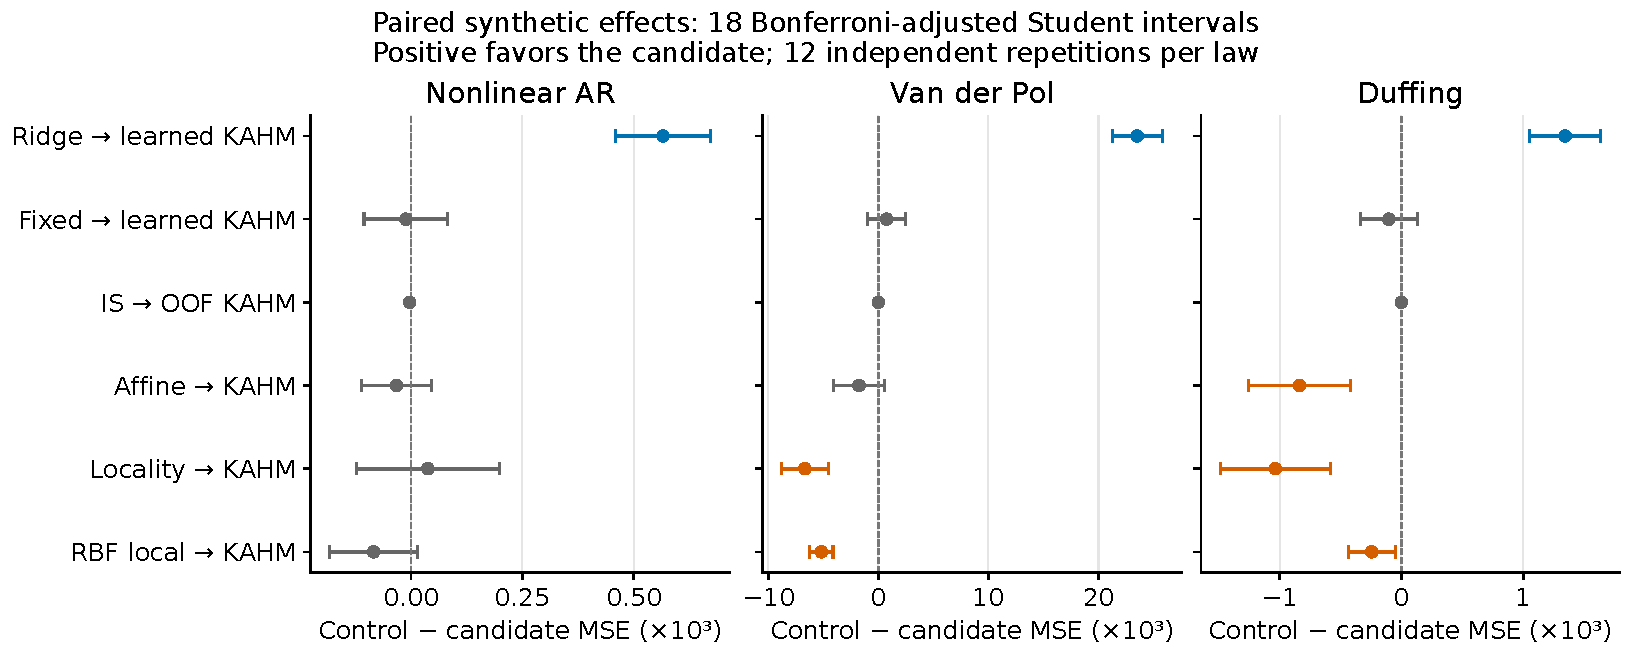
\includegraphics[width=\linewidth]{generated/target_geometry/synthetic_contrasts.pdf}
\caption{All six prescribed contrasts for each known synthetic law.
Points are paired mean differences in MSE, multiplied by $10^3$;
positive values favor the candidate named to the right of each arrow.
Intervals use the common 18-comparison Bonferroni adjustment and
12 independent repetition differences per law. The learned-metric
comparison holds OOF targets fixed; the residual-target comparison
holds the identity metric fixed. Matched-geometry comparisons use
the shared learned metric and OOF targets. Each panel has its own
horizontal range, and intervals containing zero are unresolved,
not evidence of equal performance.}
\label{fig:target-synthetic-contrasts}
\end{figure}

% Generated only from audited target-geometry predictions; no fitting.
\begin{table}[!htbp]
\centering\scriptsize\setlength{\tabcolsep}{4pt}
\caption{The complete family of 18 prespecified synthetic comparisons. $\Delta$ is control minus candidate test MSE; positive values favor the candidate. Intervals use the paired repetition differences, Student's $t_{11}$ quantile, and a two-sided Bonferroni allocation of $0.05/18$. Family coverage is approximate because normality of repetition differences is not guaranteed. No claim joins this family to earlier experiments.}
\label{tab:target-synthetic-intervals}
\begin{tabular}{lllrr}
\toprule
Law & Control & Candidate & $\Delta\times10^3$ & Family interval \\
\midrule
Nonlinear AR & Raw ridge & Learned, OOF KAHM & 0.566 & [0.459, 0.672] \\
Nonlinear AR & Fixed, OOF KAHM & Learned, OOF KAHM & -0.011 & [-0.105, 0.083] \\
Nonlinear AR & Fixed, IS KAHM & Fixed, OOF KAHM & -0.003 & [-0.006, $4.07\times10^{-4}$] \\
Nonlinear AR & Learned, OOF Affine & Learned, OOF KAHM & -0.032 & [-0.111, 0.046] \\
Nonlinear AR & Learned, OOF Locality & Learned, OOF KAHM & 0.038 & [-0.122, 0.199] \\
Nonlinear AR & Learned, OOF RBF local & Learned, OOF KAHM & -0.083 & [-0.182, 0.015] \\
Van der Pol & Raw ridge & Learned, OOF KAHM & 23.510 & [21.236, 25.785] \\
Van der Pol & Fixed, OOF KAHM & Learned, OOF KAHM & 0.754 & [-0.939, 2.447] \\
Van der Pol & Fixed, IS KAHM & Fixed, OOF KAHM & -0.003 & [-0.008, 0.002] \\
Van der Pol & Learned, OOF Affine & Learned, OOF KAHM & -1.751 & [-4.088, 0.586] \\
Van der Pol & Learned, OOF Locality & Learned, OOF KAHM & -6.661 & [-8.765, -4.558] \\
Van der Pol & Learned, OOF RBF local & Learned, OOF KAHM & -5.169 & [-6.229, -4.110] \\
Duffing & Raw ridge & Learned, OOF KAHM & 1.344 & [1.054, 1.634] \\
Duffing & Fixed, OOF KAHM & Learned, OOF KAHM & -0.103 & [-0.336, 0.130] \\
Duffing & Fixed, IS KAHM & Fixed, OOF KAHM & -0.001 & [-0.006, 0.004] \\
Duffing & Learned, OOF Affine & Learned, OOF KAHM & -0.836 & [-1.254, -0.418] \\
Duffing & Learned, OOF Locality & Learned, OOF KAHM & -1.036 & [-1.489, -0.583] \\
Duffing & Learned, OOF RBF local & Learned, OOF KAHM & -0.243 & [-0.435, -0.051] \\
\bottomrule
\end{tabular}
\end{table}

% Generated only from audited target-geometry predictions; no fitting.
\begin{table}[!htbp]
\centering\small\setlength{\tabcolsep}{4pt}
\caption{Scaled MSE by collection, averaging its three declared series. Collections receive equal weights in the aggregate; neither series nor repeated origins increase the collection count. No confidence intervals are attached to these four descriptive collection means.}
\label{tab:target-archive-sources}
\begin{tabular}{lrrrr}
\toprule
Procedure & Electricity & Bitcoin & Pedestrian & Air quality \\
\midrule
Raw ridge & 0.2879 & 3.0946 & 1.2489 & 0.5704 \\
Raw RBF & 0.2969 & 5.8096 & 1.0650 & 0.6216 \\
Persistence / seasonal naive & 0.7859 & 3.3622 & 1.5349 & 1.7073 \\
Joint raw + KAHM & 0.2760 & 3.8872 & 1.0713 & 0.5773 \\
Fixed, IS KAHM & 0.2725 & 3.0163 & 1.1943 & 0.5752 \\
Fixed, IS Affine & 0.2753 & 3.0013 & 1.1862 & 0.5708 \\
Fixed, IS Locality & 0.2678 & 3.0174 & 1.1882 & 0.5808 \\
Fixed, IS RBF local & 0.2885 & 3.0102 & 1.1697 & 0.5631 \\
Fixed, OOF KAHM & 0.2778 & 3.0781 & 1.1766 & 0.5741 \\
Fixed, OOF Affine & 0.2798 & 3.0762 & 1.1636 & 0.5728 \\
Fixed, OOF Locality & 0.2713 & 3.0559 & 1.1781 & 0.5887 \\
Fixed, OOF RBF local & 0.2828 & 3.0424 & 1.2035 & 0.5695 \\
Learned, OOF KAHM & 0.2766 & 3.0520 & 1.1943 & 0.5656 \\
Learned, OOF Affine & 0.2975 & 3.0369 & 1.1691 & 0.5711 \\
Learned, OOF Locality & 0.2751 & 3.0615 & 1.1597 & 0.5714 \\
Learned, OOF RBF local & 0.2838 & 3.0506 & 1.2278 & 0.5772 \\
\bottomrule
\end{tabular}
\end{table}

% Generated only from audited target-geometry predictions; no fitting.
\begin{table}[!htbp]
\centering\scriptsize\setlength{\tabcolsep}{4pt}
\caption{Exact natural-series roster, selected before forecasts by a salted hash among training-prefix-eligible candidates. $L$ is history length and $H$ the complete forecast path length. Chronological boundaries are 60/20/20; windows with missing inputs or targets are omitted without imputation. At most 512/64/64 windows are retained by the frozen deterministic sampling rule. The loss scale is computed before validation. Bitcoin series are network indicators, not prices.}
\label{tab:target-archive-windows}
\begin{tabular}{llrrrr}
\toprule
Collection & Series & $L$ & $H$ & Train/val/test & Loss scale \\
\midrule
Australian electricity & T3 & 48 & 12 & 512/64/64 & $1.43\times10^{5}$ \\
Australian electricity & T5 & 48 & 12 & 512/64/64 & 4182.897 \\
Australian electricity & T1 & 48 & 12 & 512/64/64 & $4.50\times10^{5}$ \\
Bitcoin indicators & sent\_addresses & 28 & 7 & 512/64/64 & $2.07\times10^{8}$ \\
Bitcoin indicators & confirmation\_time & 28 & 7 & 512/64/64 & 163.705 \\
Bitcoin indicators & block\_size & 28 & 7 & 512/64/64 & $3.19\times10^{9}$ \\
Pedestrian counts & T10 & 48 & 6 & 512/64/64 & 26088.371 \\
Pedestrian counts & T14 & 48 & 6 & 512/64/64 & 31655.986 \\
Pedestrian counts & T20 & 48 & 6 & 512/64/64 & 27784.521 \\
KDD air quality & T239 & 48 & 6 & 512/64/64 & 102.986 \\
KDD air quality & T99 & 48 & 6 & 512/64/64 & 226.458 \\
KDD air quality & T233 & 48 & 6 & 512/64/64 & 441.826 \\
\bottomrule
\end{tabular}
\end{table}

% Generated only from audited target-geometry predictions; no fitting.
\begin{table}[!htbp]
\centering\scriptsize\setlength{\tabcolsep}{4pt}
\caption{Training diagnostics, not independent evidence of test benefit. $\mathcal J$ is the regularized Gaussian residual-regression proxy shared by all geometric arms. $\mathcal J_0$ and $\mathcal J_{\rm fit}$ are the identity-metric and selected fitted-metric objectives. A finite improved iterate may be retained at an iteration limit, separately from optimizer convergence. $D$ is mean squared disagreement between donor and final ridge predictions on the same correction rows; $R_{\rm OOF}$ is their out-of-fold (OOF) residual MSE. Medians summarize observed tasks and are descriptive. Exact objectives, warnings, weight ratios, missing diagnostics and residual identities are retained in the report CSV files.}
\label{tab:target-diagnostics}
\begin{tabular}{lrrrrr}
\toprule
Phase & Tasks & Converged & Metric fallback & Median $\mathcal J_0-\mathcal J_{\rm fit}$ & Median $D/R_{\rm OOF}$ \\
\midrule
Synthetic & 36 & 36 & 0 & $1.874\times10^{-6}$ & 0.0024 \\
Archive & 12 & 12 & 0 & 0.0003 & 0.1047 \\
\bottomrule
\end{tabular}
\end{table}

% Generated only from audited target-geometry predictions; no fitting.
\begin{table}[!htbp]
\centering\scriptsize\setlength{\tabcolsep}{4pt}
\caption{Validation-selected correction strengths, with counts ordered as $\gamma=0,0.25,0.5,1$. A zero correction is the exact deployed ridge predictor. A failed arm is recorded separately as a baseline fallback, not as an observed zero-strength validation selection. Selection counts summarize tasks and do not supply an additional inference sample.}
\label{tab:target-selection}
\begin{tabular}{lrrrr}
\toprule
Procedure & Synthetic gamma counts & Fallback & Archive gamma counts & Fallback \\
\midrule
Fixed, IS KAHM & 0 / 0 / 0 / 36 & 0 & 1 / 5 / 1 / 5 & 0 \\
Fixed, IS Affine & 0 / 0 / 1 / 35 & 0 & 2 / 3 / 2 / 5 & 0 \\
Fixed, IS Locality & 0 / 0 / 1 / 35 & 0 & 0 / 3 / 5 / 4 & 0 \\
Fixed, IS RBF local & 0 / 0 / 0 / 36 & 0 & 0 / 3 / 5 / 4 & 0 \\
Fixed, OOF KAHM & 0 / 0 / 0 / 36 & 0 & 2 / 5 / 2 / 3 & 0 \\
Fixed, OOF Affine & 0 / 0 / 1 / 35 & 0 & 3 / 4 / 4 / 1 & 0 \\
Fixed, OOF Locality & 0 / 0 / 1 / 35 & 0 & 0 / 7 / 4 / 1 & 0 \\
Fixed, OOF RBF local & 0 / 0 / 0 / 36 & 0 & 1 / 4 / 6 / 1 & 0 \\
Learned, OOF KAHM & 0 / 0 / 1 / 35 & 0 & 1 / 4 / 6 / 1 & 0 \\
Learned, OOF Affine & 0 / 0 / 1 / 35 & 0 & 1 / 4 / 5 / 2 & 0 \\
Learned, OOF Locality & 0 / 0 / 1 / 35 & 0 & 1 / 4 / 7 / 0 & 0 \\
Learned, OOF RBF local & 0 / 0 / 0 / 36 & 0 & 0 / 5 / 5 / 2 & 0 \\
\bottomrule
\end{tabular}
\end{table}

% Generated only from audited target-geometry predictions; no fitting.
\begin{table}[!htbp]
\centering\small\setlength{\tabcolsep}{4pt}
\caption{Descriptive sensitivity to collection composition: each column omits the named collection and recomputes the mean scaled loss over the remaining three collections, divided by the corresponding raw-ridge loss. Values below one favor the procedure. Every omission is shown; none is selected as the primary result. These ratios are not independent replications, confidence intervals, or additional confirmatory tests.}
\label{tab:target-leave-one-source-out}
\begin{tabular}{lrrrr}
\toprule
Procedure & Electricity & Bitcoin & Pedestrian & Air quality \\
\midrule
Raw ridge & 1.000 & 1.000 & 1.000 & 1.000 \\
Raw RBF & 1.526 & 0.941 & 1.702 & 1.548 \\
Persistence / seasonal naive & 1.344 & 1.912 & 1.481 & 1.227 \\
Joint raw + KAHM & 1.127 & 0.913 & 1.199 & 1.130 \\
Fixed, IS KAHM & 0.974 & 0.969 & 0.977 & 0.968 \\
Fixed, IS Affine & 0.968 & 0.964 & 0.973 & 0.964 \\
Fixed, IS Locality & 0.974 & 0.967 & 0.978 & 0.966 \\
Fixed, IS RBF local & 0.965 & 0.959 & 0.977 & 0.965 \\
Fixed, OOF KAHM & 0.983 & 0.963 & 0.994 & 0.979 \\
Fixed, OOF Affine & 0.979 & 0.957 & 0.994 & 0.976 \\
Fixed, OOF Locality & 0.981 & 0.967 & 0.991 & 0.973 \\
Fixed, OOF RBF local & 0.980 & 0.976 & 0.985 & 0.978 \\
Learned, OOF KAHM & 0.979 & 0.966 & 0.985 & 0.977 \\
Learned, OOF Affine & 0.972 & 0.967 & 0.988 & 0.972 \\
Learned, OOF Locality & 0.975 & 0.952 & 0.989 & 0.971 \\
Learned, OOF RBF local & 0.988 & 0.991 & 0.990 & 0.985 \\
\bottomrule
\end{tabular}
\end{table}

\FloatBarrier
